\documentclass[aspectratio=169,11pt]{beamer}

% --- packages ----------------------------------------------------------------
\usepackage{mathptmx}             % Times New Roman
\usepackage[T1]{fontenc}
\usepackage[utf8]{inputenc}
\usepackage[expansion=false]{microtype}
\usepackage{graphicx}
\usepackage{booktabs}
\usepackage{tabularx}
\usepackage{array}
\usepackage{xcolor}
\usepackage{tikz}
\usetikzlibrary{positioning,arrows.meta,shapes.geometric,fit,backgrounds}

% --- minimalist academic theme ----------------------------------------------
\definecolor{slate}{HTML}{1F3A5F}
\definecolor{accent}{HTML}{B5651D}
\definecolor{ec2blue}{HTML}{1F77B4}
\definecolor{fgreen}{HTML}{2CA02C}
\definecolor{lambdared}{HTML}{D62728}
\definecolor{neutralgrey}{HTML}{555555}
\definecolor{lightgrey}{HTML}{F0F0F0}

\usecolortheme{default}
\setbeamercolor{normal text}{fg=black,bg=white}
\setbeamercolor{title}{fg=slate}
\setbeamercolor{frametitle}{fg=slate,bg=white}
\setbeamercolor{structure}{fg=slate}
\setbeamercolor{section in toc}{fg=slate}
\setbeamercolor{author}{fg=black!75}
\setbeamercolor{institute}{fg=black!55}
\setbeamercolor{date}{fg=black!55}
\setbeamercolor{itemize item}{fg=accent}
\setbeamercolor{itemize subitem}{fg=accent}
\setbeamercolor{block title}{fg=white,bg=slate}
\setbeamercolor{block body}{bg=lightgrey}

\setbeamerfont{title}{series=\bfseries,size=\Large}
\setbeamerfont{subtitle}{series=\mdseries,size=\normalsize,shape=\itshape}
\setbeamerfont{frametitle}{series=\bfseries,size=\large}
\setbeamerfont{author}{series=\mdseries,size=\small}
\setbeamerfont{institute}{series=\mdseries,size=\footnotesize,shape=\itshape}

\setbeamertemplate{navigation symbols}{}
\setbeamertemplate{itemize item}{\textbullet}
\setbeamertemplate{frametitle}{%
  \vspace{6pt}\hspace{8pt}%
  {\usebeamercolor[fg]{frametitle}\usebeamerfont{frametitle}\insertframetitle}\par%
  \vspace{-2pt}\hspace{8pt}\textcolor{slate!40}{\rule{\dimexpr\paperwidth-16pt\relax}{0.6pt}}\par
}
\setbeamertemplate{footline}{%
  \vskip 2pt%
  \hbox to \paperwidth{%
    \hspace*{14pt}%
    \scriptsize\textcolor{black!45}{CS5296 Group~24}%
    \hfil%
    \scriptsize\textcolor{black!45}{\insertframenumber\,/\,\inserttotalframenumber}%
    \hspace*{14pt}%
  }%
  \vskip 6pt%
}

\setbeamersize{text margin left=18pt,text margin right=18pt}
\renewcommand{\baselinestretch}{1.05}

% --- title metadata ----------------------------------------------------------
\title{A Controlled, End-to-End Comparison of \\ EC2, ECS Fargate, and AWS Lambda}
\subtitle{for Stateless Web Services}
\author{Ma Liyu \and Zheng Junlan \and Zheng Zelan}
\institute{CS5296 Cloud Computing, Spring 2026 \\ City University of Hong Kong, Group~24}
\date{April 2026}

\begin{document}

% =============================================================================
% SLIDE 1 -- TITLE
% =============================================================================
\begin{frame}[plain]
  \vspace{20pt}
  \begin{center}
    {\usebeamercolor[fg]{title}\usebeamerfont{title}\inserttitle}\\[6pt]
    {\usebeamercolor[fg]{title}\usebeamerfont{subtitle}\insertsubtitle}\\[28pt]

    {\usebeamerfont{author}Ma~Liyu \quad Zheng~Junlan \quad Zheng~Zelan}\\[6pt]
    {\usebeamercolor[fg]{institute}\usebeamerfont{institute}\insertinstitute}\\[20pt]
    {\usebeamercolor[fg]{date}\usebeamerfont{institute}\insertdate}
  \end{center}

  \vfill
  \begin{center}
    \scriptsize\textcolor{black!55}{\href{https://github.com/Fighterforever/cs5296}{github.com/Fighterforever/cs5296}}
  \end{center}
\end{frame}

% =============================================================================
% SLIDE 2 -- THE CHOICE PROBLEM
% =============================================================================
\begin{frame}{Three ways to run the same web service on AWS}
  \vspace{4pt}
  \begin{columns}[T,onlytextwidth]
    \begin{column}{0.32\linewidth}
      \begin{block}{\textcolor{white}{EC2}}
        Virtual machines.\\[2pt]
        Predictable performance.\\[2pt]
        \emph{You} handle scaling and OS upkeep.\\[6pt]
        Billed by the running hour.
      \end{block}
    \end{column}
    \begin{column}{0.32\linewidth}
      \begin{block}{\textcolor{white}{ECS Fargate}}
        Managed containers.\\[2pt]
        AWS handles the host.\\[2pt]
        \emph{Your} task definition decides the size.\\[6pt]
        Billed by the vCPU-second.
      \end{block}
    \end{column}
    \begin{column}{0.32\linewidth}
      \begin{block}{\textcolor{white}{AWS Lambda}}
        Functions on demand.\\[2pt]
        No servers, no idle cost.\\[2pt]
        Cold-start penalty after idle.\\[6pt]
        Billed per request \(+\) per~GB-second.
      \end{block}
    \end{column}
  \end{columns}

  \vspace{18pt}
  \begin{center}
    \emph{Performance, elasticity, and cost rarely move in the same direction.}\\[2pt]
    \emph{Most public studies compare different applications. We compare them apples to apples.}
  \end{center}
\end{frame}

% =============================================================================
% SLIDE 3 -- ARCHITECTURE: ONE IMAGE, THREE RUNTIMES
% =============================================================================
\begin{frame}{One container image, three runtimes, one ALB}
  \vspace{-2pt}
  \begin{center}
  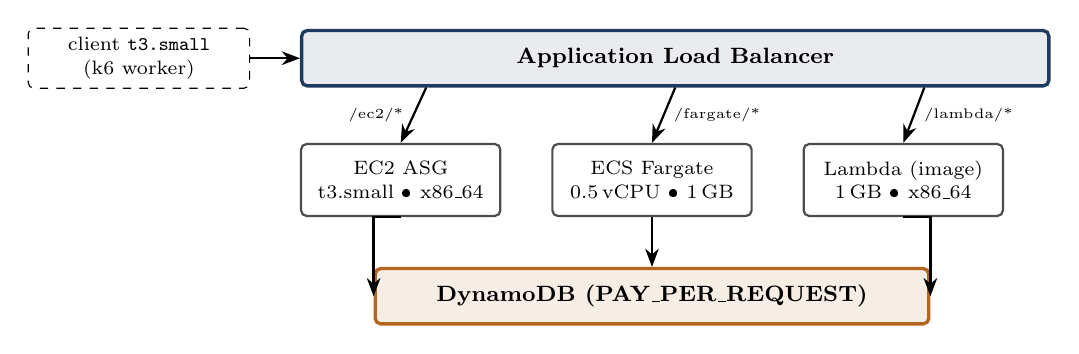
\begin{tikzpicture}[
    font=\scriptsize,
    node distance=8pt and 18pt,
    box/.style={draw=black!70, thick, rounded corners=2pt, align=center,
                minimum width=72pt, minimum height=26pt, fill=white},
    alb/.style={draw=slate, very thick, fill=slate!10, rounded corners=2pt,
                minimum width=270pt, minimum height=20pt, align=center, font=\footnotesize\bfseries},
    ddb/.style={draw=accent, very thick, fill=accent!12, rounded corners=2pt,
                minimum width=200pt, minimum height=20pt, align=center, font=\footnotesize\bfseries},
    client/.style={draw=black, dashed, rounded corners=2pt, minimum width=80pt,
                   minimum height=20pt, align=center},
    arrow/.style={-{Stealth}, thick},
  ]
    \node[client] (cl) {client \texttt{t3.small}\\(k6 worker)};
    \node[alb, right=of cl] (alb) {Application Load Balancer};
    \node[box, below=20pt of alb.south west, anchor=north west] (ec2)
       {EC2 ASG\\\scriptsize t3.small \textbullet{} x86\_64};
    \node[box, right=of ec2] (fg)
       {ECS Fargate\\\scriptsize 0.5\,vCPU \textbullet{} 1\,GB};
    \node[box, right=of fg] (lam)
       {Lambda (image)\\\scriptsize 1\,GB \textbullet{} x86\_64};
    \node[ddb, below=18pt of fg] (ddb) {DynamoDB (PAY\_PER\_REQUEST)};

    \draw[arrow] (cl) -- (alb);
    \draw[arrow] (alb.south) ++(-90pt,0) -- node[left,font=\tiny]{/ec2/*}     (ec2.north);
    \draw[arrow] (alb.south)              -- node[right,font=\tiny]{/fargate/*} (fg.north);
    \draw[arrow] (alb.south) ++( 90pt,0) -- node[right,font=\tiny]{/lambda/*} (lam.north);
    \draw[arrow] (ec2.south) -- (ddb.west |- ec2.south) -- (ddb.west);
    \draw[arrow] (fg.south)  -- (ddb.north);
    \draw[arrow] (lam.south) -- (ddb.east |- lam.south) -- (ddb.east);
  \end{tikzpicture}
  \end{center}

  \vspace{4pt}
  \begin{itemize}\setlength\itemsep{2pt}
    \item Same OCI image (\texttt{shortlink:v2}) deployed unmodified to all three.
    \item Lambda runs the same image via the AWS Lambda Web Adapter, translating invocations into HTTP calls to localhost.
    \item Shared backend (DynamoDB) and shared frontend (ALB) confine measurable differences to the compute layer.
  \end{itemize}
\end{frame}

% =============================================================================
% SLIDE 4 -- FOUR SCENARIOS
% =============================================================================
\begin{frame}{Four scenarios, driven by the same k6 harness}
  \vspace{4pt}
  \footnotesize
  \renewcommand{\arraystretch}{1.35}
  \begin{tabular}{@{}p{0.22\linewidth}@{\hspace{8pt}}p{0.74\linewidth}@{}}
    \textcolor{slate}{\bfseries Steady-state}    & Constant arrival rate. EC2 and Fargate: 50/100/200/400\,RPS. Lambda: 25/50/75\,RPS. Recovers per-stage tail latency. \\
    \textcolor{slate}{\bfseries Step burst}      & One minute idle, three minutes at the target rate, one minute idle. Captures elasticity and time-to-steady-state. \\
    \textcolor{slate}{\bfseries Cold-start probe} & Twelve sparse \texttt{/healthz} requests with 60-second gaps. Designed to characterise warm-vs-cold latency on Lambda. \\
    \textcolor{slate}{\bfseries Mixed R/W}       & 70\,\% GET-redirect, 30\,\% POST-shorten at 200\,RPS for three minutes. Approximates a real shortener mix. \\
  \end{tabular}

  \vspace{12pt}
  \begin{center}
    \scriptsize\textcolor{black!55}{All scenarios driven from a co-located \texttt{t3.small} k6 worker in \texttt{us-east-1a}; bootstrap 95\,\% CIs on every reported percentile.}
  \end{center}
\end{frame}

% =============================================================================
% SLIDE 5 -- STEADY-STATE RESULTS
% =============================================================================
\begin{frame}{Steady-state: Lambda is flat, EC2 has a fat tail, Fargate saturates}
  \begin{columns}[T]
    \begin{column}{0.62\linewidth}
      \vspace{-4pt}
      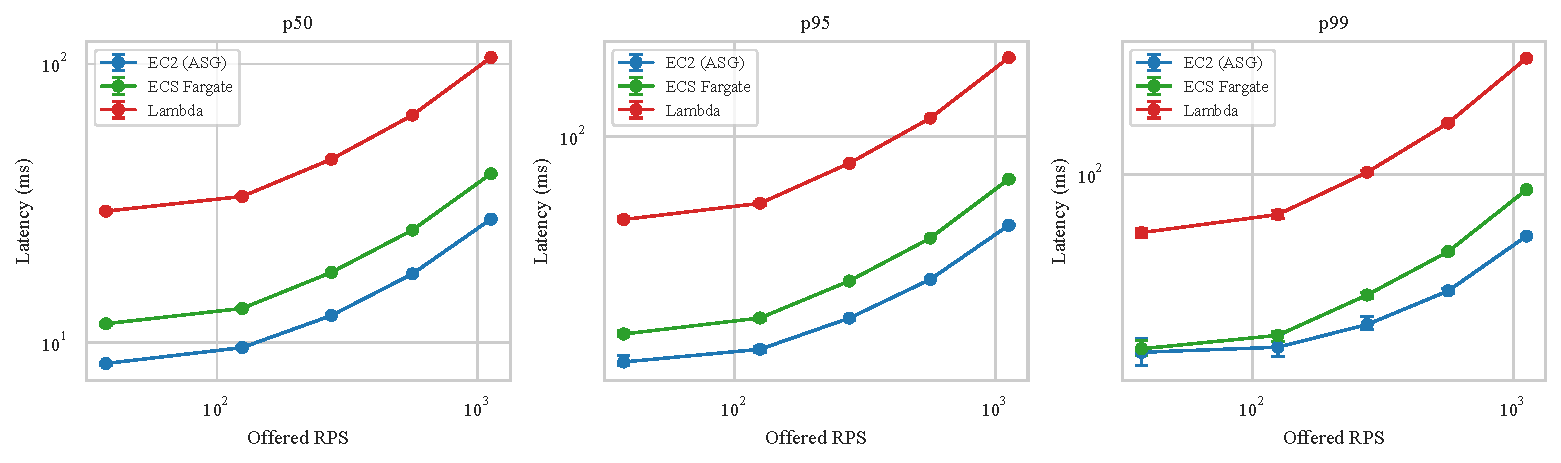
\includegraphics[width=\linewidth]{figures/steady_latency_vs_rps}
    \end{column}
    \begin{column}{0.36\linewidth}
      \footnotesize
      \textbf{\textcolor{lambdared}{Lambda (1\,GB)}}\\
      p50 $\approx$ 29\,ms,
      p95 $\approx$ 40\,ms,
      p99 $\approx$ 52\,ms across the entire band.\\[6pt]

      \textbf{\textcolor{ec2blue}{EC2 (t3.small ASG)}}\\
      Tight 13\,ms median up to 200\,RPS. p95 goes from 26\,ms to over 600\,ms as the burstable-credit budget runs out.\\[6pt]

      \textbf{\textcolor{fgreen}{Fargate (0.5\,vCPU)}}\\
      Saturates by 100\,RPS. At 400\,RPS, 6.9\,\% of requests hit the ALB idle timeout.
    \end{column}
  \end{columns}
\end{frame}

% =============================================================================
% SLIDE 6 -- ELASTICITY UNDER BURST
% =============================================================================
\begin{frame}{Elasticity: per-second p95 through a 3-minute burst}
  \begin{columns}[T]
    \begin{column}{0.66\linewidth}
      \vspace{-4pt}
      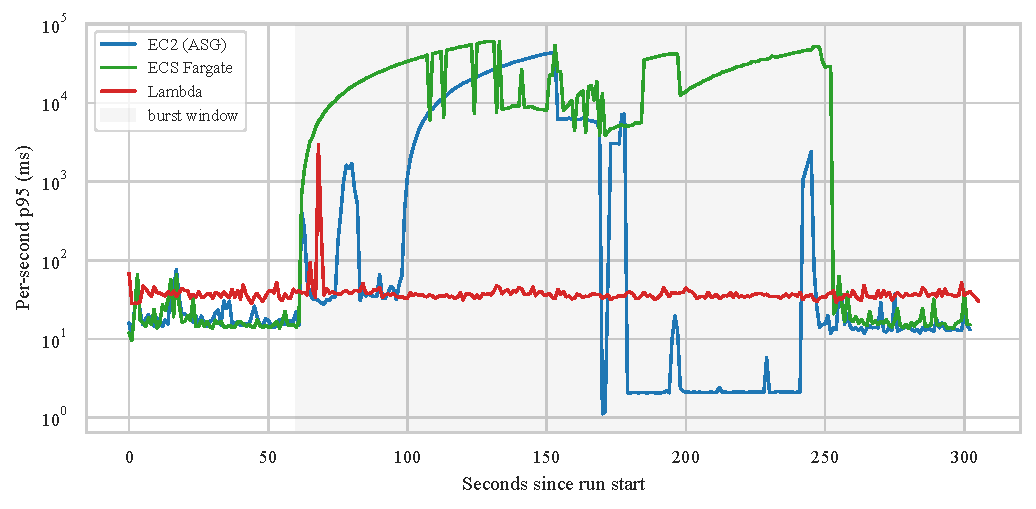
\includegraphics[width=\linewidth]{figures/elasticity_p95_trace}
    \end{column}
    \begin{column}{0.32\linewidth}
      \footnotesize
      \vspace{18pt}
      \textbf{\textcolor{lambdared}{Lambda}} \,—\, tracks its steady envelope from the first second.\\[10pt]

      \textbf{\textcolor{ec2blue}{EC2}} \,—\, takes about a minute for the second ASG instance to come online and rejoin the load balancer.\\[10pt]

      \textbf{\textcolor{fgreen}{Fargate}} \,—\, the single task collapses; ECS service autoscaling at the default 30-second cooldown is too slow to recover.
    \end{column}
  \end{columns}
\end{frame}

% =============================================================================
% SLIDE 7 -- COST AND BREAK-EVEN
% =============================================================================
\begin{frame}{Cost: a single break-even crossover near 20 RPS}
  \begin{columns}[T]
    \begin{column}{0.56\linewidth}
      \vspace{-2pt}
      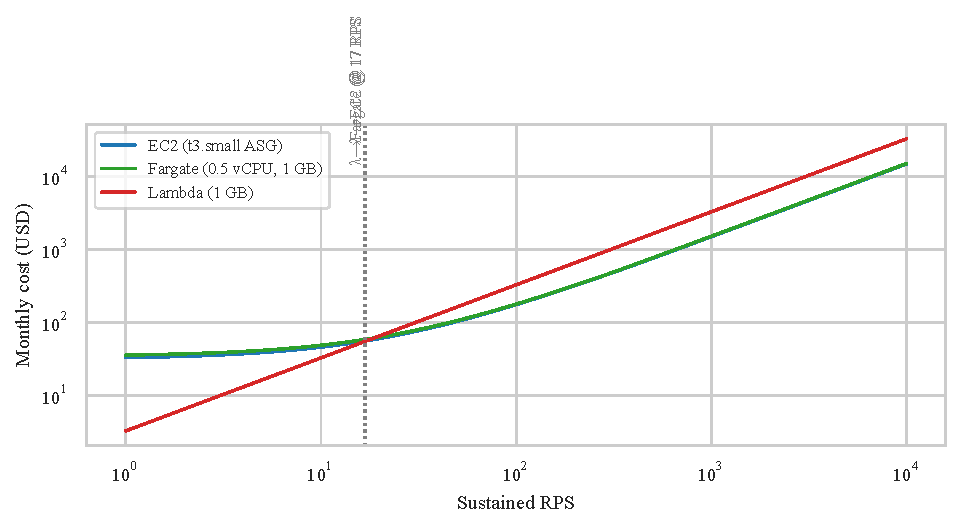
\includegraphics[width=\linewidth]{figures/cost_vs_rps}
    \end{column}
    \begin{column}{0.42\linewidth}
      \vspace{-2pt}
      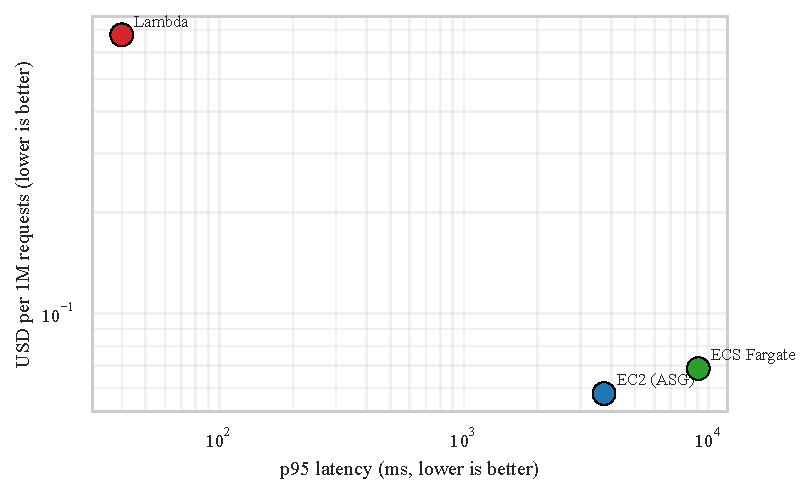
\includegraphics[width=\linewidth]{figures/cost_latency_pareto}
    \end{column}
  \end{columns}

  \vspace{4pt}
  \footnotesize
  \begin{itemize}\setlength\itemsep{1pt}\setlength\topsep{0pt}
    \item Below \(\sim\)20\,RPS Lambda wins (no idle cost); above it pre-provisioned compute amortises enough.
    \item At 50\,RPS Lambda is \emph{Pareto-dominant} on both axes in our measured regime.
  \end{itemize}
\end{frame}

% =============================================================================
% SLIDE 8 -- LIVE DEMO TRANSITION
% =============================================================================
\begin{frame}[plain]
  \vfill
  \begin{center}
    {\usebeamercolor[fg]{title}\usebeamerfont{title}Live demo}\\[10pt]
    {\itshape Deployment, benchmark harness, and reproduction.}
  \end{center}
  \vfill
\end{frame}

% =============================================================================
% SLIDE 9 -- REPRODUCIBILITY
% =============================================================================
\begin{frame}{Reproducibility in five \texttt{make} targets}
  \vspace{4pt}
  \begin{block}{One repo, one command per phase}
    \texttt{git clone https://github.com/Fighterforever/cs5296.git \&\& cd cs5296}\\[4pt]
    \begin{tabular}{ll}
      \texttt{make image}    & build the OCI container image (\texttt{linux/amd64}, multi-runtime) \\
      \texttt{make up}       & \texttt{tofu apply}: 39 AWS resources in $\sim$7 minutes \\
      \texttt{make bench}    & drive the 4-scenario k6 matrix against the live ALB \\
      \texttt{make analyze}  & bootstrap stats, write 5 figures and 4 CSV summaries \\
      \texttt{make report}   & compile the LaTeX report end-to-end \\
      \texttt{make nuke}     & destroy + sweep stray ENI/EIP \\
    \end{tabular}
  \end{block}

  \vspace{4pt}
  \begin{itemize}\setlength\itemsep{2pt}
    \item Infrastructure-as-code in OpenTofu/Terraform; portable to any AWS account.
    \item Analysis pipeline in Python; figures regenerate from raw k6 CSV in under a minute.
    \item Total measured AWS spend for one full matrix run: \,$<$\,\$1.
  \end{itemize}
\end{frame}

% =============================================================================
% SLIDE 10 -- FINDINGS AND THREATS
% =============================================================================
\begin{frame}{Three findings, two honest threats to validity}
  \begin{columns}[T]
    \begin{column}{0.52\linewidth}
      \textbf{Findings}\\[2pt]
      \begin{enumerate}[1.]\setlength\itemsep{4pt}
        \item Lambda dominates up to \(\sim\)20\,RPS \,—\, no-idle billing plus the most stable tail in the measured band.
        \item EC2 keeps a tight median further than expected (200\,RPS), but its tail blows out once the burstable-credit budget is depleted.
        \item Fargate at the smallest size is \emph{not} Lambda-with-containers \,—\, a single 0.5\,vCPU task cannot absorb 100\,RPS of Python.
      \end{enumerate}
    \end{column}
    \begin{column}{0.46\linewidth}
      \textbf{Threats to validity}\\[2pt]
      \begin{itemize}\setlength\itemsep{4pt}
        \item Cold-start probe used 60-second gaps, too short to reliably reclaim Lambda containers (typical reclaim 5--15\,min). All probe samples landed in the warm band; one genuine cold start (4.3\,s) captured incidentally.
        \item New AWS account default Lambda concurrency was 10; this capped our Lambda peak at 75\,RPS. A quota-increase ticket would lift it.
      \end{itemize}
    \end{column}
  \end{columns}
\end{frame}

% =============================================================================
% SLIDE 11 -- THANK YOU
% =============================================================================
\begin{frame}[plain]
  \vfill
  \begin{center}
    {\usebeamercolor[fg]{title}\usebeamerfont{title}Thank you}\\[18pt]

    {\large Code, raw measurements, figures, and the report are public:}\\[8pt]
    {\large\ttfamily github.com/Fighterforever/cs5296}\\[26pt]

    \footnotesize\textcolor{black!60}{Group~24 \,\textbar\, CS5296 Cloud Computing, Spring 2026 \,\textbar\, City University of Hong Kong}
  \end{center}
  \vfill
\end{frame}

\end{document}
